\documentclass[a4paper,12pt]{article}
\usepackage[utf8]{inputenc}
\usepackage{amsmath}
\usepackage{amssymb}
\usepackage{graphicx}
\usepackage{geometry}
\usepackage{tikz}
\usepackage{pgfplots}
\pgfplotsset{width=9cm, compat=1.9}
\usepackage{multicol}
\usepackage{array}
\setlength{\columnsep}{1cm}
\usepackage[inline]{enumitem}
\usepackage{setspace}
\usepackage{subcaption}
\usepackage{array}
\newcolumntype{L}[1]{>{\raggedright\let\newline\\\arraybackslash\hspace{0pt}}m{#1}}
\newcolumntype{C}[1]{>{\centering\let\newline\\\arraybackslash\hspace{0pt}}m{#1}}
\newcolumntype{R}[1]{>{\raggedleft\let\newline\\\arraybackslash\hspace{0pt}}m{#1}}
\usepackage{tcolorbox}
\usepackage{listofitems}
\renewcommand{\arraystretch}{1.5}
\geometry{a4paper, margin=1.5cm}
\setlength\parindent{0pt}
\newcommand\boxes[7]{
\begin{tikzpicture}
\newcommand{\wid}{1.6cm}
\newcommand{\hgt}{1cm}
\newcommand{\brd}{0.4cm}
\draw[](0,0)rectangle(0+\wid,0+\hgt);
\draw[](\wid/2,\hgt/2)node[]{#1};
\draw[](0-\wid/2,0-\hgt)rectangle(0+\wid/2,0);
\draw[](0,-\hgt/2)node[]{#2};
\draw[](0+\wid/2,0-\hgt)rectangle(0+3*\wid/2,0);
\draw[](\wid,-\hgt/2)node[]{#3};
\draw[](0-\wid,0-2*\hgt)rectangle(0,-\hgt);
\draw[](-\wid/2,-3*\hgt/2)node[]{#4};
\draw[](0,0-2*\hgt)rectangle(\wid,-\hgt);
\draw[](\wid/2,-3*\hgt/2)node[]{#5};
\draw[](0+\wid,0-2*\hgt)rectangle(2*\wid,-\hgt);
\draw[](3*\wid/2,-3*\hgt/2)node[]{#6};
\draw[white](-\wid-\brd,-2*\hgt-\brd)rectangle(2*\wid+\brd,\hgt+\brd);
\draw[](-\wid-\brd,\hgt+\brd)node[anchor= north west]{\textbf{#7)}};
\end{tikzpicture}
}
\newcommand\boxesSols[7]{
	\begin{tikzpicture}[scale=0.75]
	\newcommand{\wid}{1.6cm}
	\newcommand{\hgt}{1cm}
	\newcommand{\brd}{0.4cm}
	\draw[](0,0)rectangle(0+\wid,0+\hgt);
	\draw[](\wid/2,\hgt/2)node[]{#1};
	\draw[](0-\wid/2,0-\hgt)rectangle(0+\wid/2,0);
	\draw[](0,-\hgt/2)node[]{#2};
	\draw[](0+\wid/2,0-\hgt)rectangle(0+3*\wid/2,0);
	\draw[](\wid,-\hgt/2)node[]{#3};
	\draw[](0-\wid,0-2*\hgt)rectangle(0,-\hgt);
	\draw[](-\wid/2,-3*\hgt/2)node[]{#4};
	\draw[](0,0-2*\hgt)rectangle(\wid,-\hgt);
	\draw[](\wid/2,-3*\hgt/2)node[]{#5};
	\draw[](0+\wid,0-2*\hgt)rectangle(2*\wid,-\hgt);
	\draw[](3*\wid/2,-3*\hgt/2)node[]{#6};
	\draw[white](-\wid-\brd,-2*\hgt-\brd)rectangle(2*\wid+\brd,\hgt+\brd);
	\draw[](-\wid-\brd,\hgt+\brd)node[anchor= north west]{\textbf{#7)}};
	\end{tikzpicture}
}
\newcommand\magicsquare[9]{
\begin{tikzpicture}
\newcommand{\wid}{1.5cm}
\newcommand{\hgt}{1.5cm}
\newcommand{\brd}{0.3cm}
\draw[](0,0)rectangle(3*\wid,3*\hgt);
\draw[pink](0-\brd,0-5*\brd)rectangle(3*\wid+5*\brd,3*\hgt+\brd);
\draw[](\wid,0)--(\wid,3*\hgt);
\draw[](2*\wid,0)--(2*\wid,3*\hgt);
\draw[](0,\hgt)--(3*\wid,\hgt);
\draw[](0,2*\hgt)--(3*\wid,2*\hgt);
\draw[](\wid/2,\hgt/2)node[]{\Large #1};
\draw[](\wid/2,3*\hgt/2)node[]{\Large #2};
\draw[](\wid/2,5*\hgt/2)node[]{\Large #3};
\draw[](3*\wid/2,\hgt/2)node[]{\Large #4};
\draw[](3*\wid/2,3*\hgt/2)node[]{\Large #5};
\draw[](3*\wid/2,5*\hgt/2)node[]{\Large #6};
\draw[](5*\wid/2,\hgt/2)node[]{\Large #7};
\draw[](5*\wid/2,3*\hgt/2)node[]{\Large #8};
\draw[](5*\wid/2,5*\hgt/2)node[]{\Large #9};
\draw(0,-0.75)node[right]{\Large \textbf{Magic Number =}};
\end{tikzpicture}
}

%first 9 arguments are  numbers for the square: row by row, top down, left to right
%numbers are separated by commas
%the 10th number is the question number
\newcommand\magicsquareA[1]{
	\setsepchar{,}
	\readlist\arg{#1} 
	\begin{tikzpicture}
	\newcommand{\wid}{1.3cm}
	\newcommand{\hgt}{1.3cm}
	\newcommand{\brd}{0.5cm}
	\draw[](0,0)rectangle(3*\wid,3*\hgt);
	\draw[](0-\brd,3*\hgt+1.2*\brd)node[anchor=north west]{\textbf{\arg[10])}};
\draw[white](0-\brd,0-2*\brd)rectangle(3*\wid+3*\brd,3*\hgt+\brd);
	\draw[](\wid,0)--(\wid,3*\hgt);
	\draw[](2*\wid,0)--(2*\wid,3*\hgt);
	\draw[](0,\hgt)--(3*\wid,\hgt);
	\draw[](0,2*\hgt)--(3*\wid,2*\hgt);
	\draw[](\wid/2,\hgt/2)node[]{\Large \arg[7]};
	\draw[](\wid/2,3*\hgt/2)node[]{\Large \arg[4]};
	\draw[](\wid/2,5*\hgt/2)node[]{\Large \arg[1]};
	\draw[](3*\wid/2,\hgt/2)node[]{\Large \arg[8]};
	\draw[](3*\wid/2,3*\hgt/2)node[]{\Large \arg[5]};
	\draw[](3*\wid/2,5*\hgt/2)node[]{\Large \arg[2]};
	\draw[](5*\wid/2,\hgt/2)node[]{\Large \arg[9]};
	\draw[](5*\wid/2,3*\hgt/2)node[]{\Large \arg[6]};
	\draw[](5*\wid/2,5*\hgt/2)node[]{\Large \arg[3]};
	\draw(0,-0.75)node[right]{\footnotesize \textbf{Magic Number =$\arg[11]$}};
	\end{tikzpicture}	
}

\newcommand\magicsquareASols[1]{
	\setsepchar{,}
	\readlist\arg{#1} 
	\begin{tikzpicture}[scale=0.75]
	\newcommand{\wid}{1.3cm}
	\newcommand{\hgt}{1.3cm}
	\newcommand{\brd}{0.5cm}
	\draw[](0,0)rectangle(3*\wid,3*\hgt);
	\draw[](0-\brd,3*\hgt+1.2*\brd)node[anchor=north west]{\textbf{\arg[10])}};
	\draw[white](0-\brd,0-2*\brd)rectangle(3*\wid+3*\brd,3*\hgt+\brd);
	\draw[](\wid,0)--(\wid,3*\hgt);
	\draw[](2*\wid,0)--(2*\wid,3*\hgt);
	\draw[](0,\hgt)--(3*\wid,\hgt);
	\draw[](0,2*\hgt)--(3*\wid,2*\hgt);
	\draw[](\wid/2,\hgt/2)node[]{\Large \arg[7]};
	\draw[](\wid/2,3*\hgt/2)node[]{\Large \arg[4]};
	\draw[](\wid/2,5*\hgt/2)node[]{\Large \arg[1]};
	\draw[](3*\wid/2,\hgt/2)node[]{\Large \arg[8]};
	\draw[](3*\wid/2,3*\hgt/2)node[]{\Large \arg[5]};
	\draw[](3*\wid/2,5*\hgt/2)node[]{\Large \arg[2]};
	\draw[](5*\wid/2,\hgt/2)node[]{\Large \arg[9]};
	\draw[](5*\wid/2,3*\hgt/2)node[]{\Large \arg[6]};
	\draw[](5*\wid/2,5*\hgt/2)node[]{\Large \arg[3]};
	\draw(0,-0.75)node[right]{\footnotesize \textbf{Magic Number =$\arg[11]$}};
	\end{tikzpicture}
}
\newcommand\baseTwoSum[1]{
$#1=\rule{7.5mm}{0.15mm} \times 2^5 + \rule{7.5mm}{0.15mm} \times 2^4 + \rule{7.5mm}{0.15mm} \times 2^3 + \rule{7.5mm}{0.15mm} \times 2^2+ \rule{7.5mm}{0.15mm} \times 2^1+ \rule{7.5mm}{0.15mm} \times 2^0$
}
\newcommand\baseTwoSumSmall[1]{
$~~~#1=\rule{7.5mm}{0.15mm} \times 2^4 + \rule{7.5mm}{0.15mm} \times 2^3 + \rule{7.5mm}{0.15mm} \times 2^2+ \rule{7.5mm}{0.15mm} \times 2^1+ \rule{7.5mm}{0.15mm} \times 2^0$
}

\newcommand\Mydiv[2]{%
$\strut#1$\kern.25em\smash{\raise.3ex\hbox{$\big)$}}$\mkern-8mu
        \overline{\enspace\strut#2}$}

\begin{document}
\thispagestyle{empty}	
\Large
\begin{figure} 
	\centering
	
\includegraphics[height=4cm]{Marsden_green_on_white.jpg}
	\caption*{February 2019}
\end{figure}
.
\vspace{3cm}
\begin{center}
	\textbf{Year 9 Number 1 Extension Booklet}
\end{center}

\vspace{3cm}

\normalsize
\newpage
\tableofcontents
\newpage

\section{General Arithmetic}
Without a calculator, work out the following
\begin{enumerate}[itemsep=10mm]
\item \begin{multicols}{3}
\begin{enumerate}[label= \roman*), itemsep=4mm]
\item $79 + 44=$
\item $98 + 63=$
\item $125 + 189=$
\item $98-57=$
\item $48 - 100=$
\item $61 -88=$
\end{enumerate}
\end{multicols}
\item \begin{multicols}{3}
\begin{enumerate}[label= \roman*), itemsep=4mm]
\item $15 \times 9 =$
\item $19 \times -7 =$
\item $-21 \times 11 =$
\item $-35 \times 14=$
\item $38 \times 24=$
\item $45 \times 16=$
\end{enumerate}
\end{multicols}
\item \begin{multicols}{3}
\begin{enumerate}[label= \roman*), itemsep=4mm]
\item $1.5 \times 2.5=$
\item $1.8 \times -1.7=$
\item $-2.1 \times 1.1=$
\item $-3.5 \times -1.2=$
\item $6 \times -2.45=$
\item $8 \times 9.9=$
\end{enumerate}
\end{multicols}
\item \begin{multicols}{3}
\begin{enumerate}[label= \roman*), itemsep=4mm]
\item $456 \div 4=$
\item \Mydiv{7}{161} 
\item $\displaystyle \frac{90}{5}=$
\item $312 \div 8=$
\item \Mydiv{14}{4914}
\item $\displaystyle \frac{112}{7}=$
\end{enumerate}
\end{multicols}
\item For these give the answer with a remainder.\\
For example $28 \div 3 = 9~~R~1$ (9 remainder 1)
\begin{multicols}{3}
\begin{enumerate}[label= \roman*), itemsep=4mm]
\item $100 \div 8=$
\item $115 \div 3=$
\item $97 \div 14=$
\item $78 \div 9=$
\item $125 \div 6=$
\item $77 \div 16=$
\end{enumerate}
\end{multicols}
\end{enumerate}
\newpage
\section{Modular Arithmetic}
\subsection{Definition}
When an integer $A$ is divided by a positive integer $N$, it has a remainder $R$ from the division.\\
The value of $R$ can be $0$ and $0\leq R < N$ (R will be greater than or equal to 0 and less than $N$).\\
We can define an operation: $$A \bmod N = R$$
Where $R$ is the remainder when $A$ is divided by $N$.\\\\
Let's look at some examples:
\begin{center}
\begin{multicols}{2}
$5 \bmod 2 = 1$\\
\tiny because $5\div 2$ has a remainder of 1 \normalsize \\
$8 \bmod 3 = 2$\\
\tiny because $8\div 3$ has a remainder of 2 \normalsize \\
$39 \bmod 7 = 4$\\
\tiny because $39\div 7$ has a remainder of 4 \normalsize \\
$99 \bmod 13 = 8$\\
\tiny because $99\div 13$ has a remainder of 8 \normalsize \\
$26 \bmod 13 = 0$\\
\tiny because $26\div 13$ has a remainder of 0 \normalsize\\
$7 \bmod 8 = 7$\\
\tiny because $7\div 8$ has a remainder of 7 \normalsize
\end{multicols}
\end{center}
\subsubsection{Without a calculator work out the following:}
\begin{center}
\begin{multicols}{2}
\begin{enumerate}[label= \roman*)]
\item $16 \bmod 5 = $\\
\item $19 \bmod 2 = $\\
\item $11 \bmod 11 = $\\
\item $38 \bmod 4 = $\\
\item $79 \bmod 6 = $\\
\item $90 \bmod 8 = $\\
\item $49 \bmod 7 = $\\
\item $69 \bmod 6 = $\\
\item $88 \bmod 7 = $\\
\item $76 \bmod 3 = $\\
\item $90 \bmod 10 = $\\
\item $101 \bmod 3 = $\\
\end{enumerate}
\end{multicols}
\end{center}
\newpage
\subsection{Modulus Relationships}
There are some interesting modulus relationships:
$$A \bmod N + B \bmod N = (A+B) \bmod N$$
$$A \bmod N \times B \bmod N = (A \times B) \bmod N$$
\subsubsection{Exercise:}
\begin{enumerate}
\item Make up a number of test cases and demonstrate to yourself that the above relationships are true.
\item Using what you have learned above, work out:
\begin{multicols}{2}
\begin{enumerate}[label= \roman*)]
\item $(16 \times 90) \bmod 5 = $\\
\item $(19 \times 89)\bmod 2 = $\\
\item $(11 \times 87) \bmod 11 = $\\
\item $(38 \times 61) \bmod 4 = $\\
\item $(79 \times 5) \bmod 6 = $\\
\item $(90 \times 8) \bmod 8 = $\\
\item $(49 \times 712872818) \bmod 7 = $\\
\item $(69 \times 7) \bmod 6 = $\\
\item $(88 \times 91) \bmod 7 = $\\
\item $(76 \times 2) \bmod 3 = $\\
\item $(90 \times 80 ) \bmod 10 = $\\
\item $(101 \times 100) \bmod 3 = $\\
\end{enumerate}
\end{multicols}
\item Using what you have learned above answer the following questions.
\begin{enumerate}[label= \roman*)]
\item What is the remainder when $48 \times 40$ is divided by $13$?
\item What is the remainder when $37 \times 41 \times 90$ is divided by $8$?
\item A number has prime factors $2,2,7,7,11,13$ what is the remainder when the number is divided by $3$
\item For the same number above, what is the remainder when the number is divided by $5$ ?
\end{enumerate}
\end{enumerate}
\newpage
\subsection{Divisibility Test for 3}
You probably know that if we want to know if a number is divisible by 3, we can add up the digits and if this sum is divisible by 3, then the number is divisible by 3.\\\\
But \textbf{why} is this true? This section is designed to give you an idea about how we can prove that this is the case.\\\\
Complete the following:
\begin{enumerate}
\item $1 \bmod 3 =$
\item $10 \bmod 3 =$
\item $100 \bmod 3 =$
\item $1000 \bmod 3 =$
\end{enumerate}
\begin{enumerate}
\item The number $492 = 4 \times 100 + 9 \times 10 + 2$\\
Show that $(4 \times 100 + 9 \times 10 + 2) \bmod 3 = (4+9+2)\bmod 3$
\item How can you tell that this number is divisible by 3??
\item What is the reminder when 83674 is divided by $3$ ?
\item Using a 4 digit number $PQRS$ can you \textbf{prove} that if the number is divisible by 3, then the sum of its digits is also divisible by 3?
\end{enumerate}
\subsection{General Questions}
\begin{enumerate}
\item What is the unit digit for the number $123^{456}$?
\item Prove that if $a^2 + b^2$ is a multiple of 3 then $a$ and $b$ are  multiples of 3.
\end{enumerate}

\newpage
\section{Exponents}
\begin{enumerate}
\item In the questions below find the value for the given letters ($x$ or $y$ or both)
\begin{enumerate}[label= \roman*)]
\item $2^{5}\times(1+2)=2^x+2^y$
\item $2^3 \times 2^4 = 2^x$
\item $(4 \times 3^4)^2 = y\times 3^x $
\item $32 \times 2^6 = 2^x$
\item $(3^2+3^2+3^2+3^2)^2 = x\times 3^y$
\item $12^3 = 2^y \times 3^x$
\end{enumerate}
\item Find the prime factors of $2^{302}+2^{303}$
\item Find the prime factors of $2^{21}+2^{17}$
\item Which pocket money system would you like (over a month only !!)? \\
Explain why.
\begin{enumerate}
\item \$10 each day.
\item \$3 on the first day, \$3.50 on the second and increasing by 50 cents each day.
\item 1 cent on the first day, 2 cents on the second day, 4 cents on the third, doubling each day.
\end{enumerate}
\item Which is larger $2^7+2^6$ or $2^8$ ?
\end{enumerate}
\newpage
\subsection{Working in base 2}
Please note that $2^1 = 2$ and $2^0 = 1$ (the reason for the second of these can be explained in class).\\\\
Any number can be written as sums of powers of 2.\\\\
For example:\vspace{-0.5cm}
\begin{align*}
7 &= 1\times 2^2 + 1\times 2^1 + 1 \times 2^0\\\\
12 &= 1\times 2^3 + 1 \times 2^2 + 0\times 2^1 + 0\times 2^0\\\\
18 &= 1\times 2^4 + 0\times 2^2 + 1\times 2^1 + 0 \times 2^0
\end{align*}
\subsubsection{For the following, fill in the blanks and remember that they can only be $0$ or $1$.}
\begin{enumerate}[label= \roman*)]
\item \baseTwoSumSmall{14}
\item \baseTwoSumSmall{19}
\item \baseTwoSumSmall{9}
\item \baseTwoSumSmall{25}
\item \baseTwoSumSmall{31}
\item \baseTwoSumSmall{20}
\end{enumerate}
If we just take the multiplying numbers (0,1) in order and drop any leading zeros, we can represent a number in \textbf{base 2}.\\
Base 2 is one of the most simple ways of representing numbers as it only uses two symbols $0$ and $1$.
In order, they represent place values of powers of 2 (instead of powers of 10 in our decimal system).
\begin{center}
$7 \equiv 111~~~(base~2)$\\
\tiny because $7= 1\times 2^2 + 1\times 2^1 + 1 \times 2^0$ \normalsize\\
$12 \equiv 1100~~~(base~2)$\\
\tiny because $12 = 1\times 2^3 + 1 \times 2^2 + 0\times 2^1 + 0\times 2^0$ \normalsize\\
$18 \equiv 1010~~~(base~2)$\\
\tiny because $18 = 1\times 2^4 + 0\times 2^2 + 1\times 2^1 + 0 \times 2^0$ \normalsize\\
\end{center}
The little sign $\equiv$ means ``equivalent to''. So the first statement above says 7 (in base 10) is equivalent to 111 (in base 2).\\\\
\textbf{Counting from 1 to 8:}
\begin{multicols}{4}
$1 \equiv 1~~~~(b~2)$\\
$2 \equiv 10~~~(b~2)$\\
$3 \equiv 11~~~~(b~2)$\\
$4 \equiv 100~~~(b~2)$\\
$5 \equiv 101~~~(b~2)$\\
$6 \equiv 110~~~(b~2)$\\
$7 \equiv 111~~~~(b~2)$\\
$8 \equiv 1000~~~(b~2)$
\end{multicols}
\subsubsection{Complete the following}
\begin{enumerate}
\item ~ \begin{multicols}{2}
\begin{enumerate}[label= \roman*)]
\item $9 \equiv \rule{7.5mm}{0.15mm}~~~~(b~2)$
\item $10 \equiv \rule{7.5mm}{0.15mm}~~~~(b~2)$
\item $15 \equiv \rule{7.5mm}{0.15mm}~~~~(b~2)$
\item $24 \equiv \rule{7.5mm}{0.15mm}~~~~(b~2)$
\item $35 \equiv \rule{7.5mm}{0.15mm}~~~~(b~2)$
\item $69 \equiv \rule{7.5mm}{0.15mm}~~~~(b~2)$
\end{enumerate}
\end{multicols}
\item ~ \begin{multicols}{2}
\begin{enumerate}[label= \roman*)]
\item $\rule{7.5mm}{0.15mm} \equiv 1001 ~~~~(b~2)$
\item $\rule{7.5mm}{0.15mm} \equiv 1101 ~~~~(b~2)$
\item $\rule{7.5mm}{0.15mm} \equiv 1010 ~~~~(b~2)$
\item $\rule{7.5mm}{0.15mm} \equiv 10000 ~~~~(b~2)$
\item $\rule{7.5mm}{0.15mm} \equiv 10101 ~~~~(b~2)$
\item $\rule{7.5mm}{0.15mm} \equiv 11111 ~~~~(b~2)$
\end{enumerate}
\end{multicols}
\end{enumerate}
\textbf{Let's consider introducing a decimal (or more correctly) a binary point.}\\\\
What do you think $1.1$ (base 2) means ? What about $1.01$ (base 2)?
\subsubsection{Complete the following}
\begin{enumerate}
\item ~ \begin{multicols}{2}
\begin{enumerate}[label= \roman*)]
\item $\rule{7.5mm}{0.15mm} \equiv 1.1 ~~~~(b~2)$
\item $\rule{7.5mm}{0.15mm} \equiv 1.01 ~~~~(b~2)$
\item $\rule{7.5mm}{0.15mm} \equiv 10.1 ~~~~(b~2)$
\item $\rule{7.5mm}{0.15mm} \equiv 100.11 ~~~~(b~2)$
\item $\rule{7.5mm}{0.15mm} \equiv 11.0101 ~~~~(b~2)$
\item $\rule{7.5mm}{0.15mm} \equiv 1.1111 ~~~~(b~2)$
\end{enumerate}
\end{multicols}
\item ~ \begin{multicols}{2}
\begin{enumerate}[label= \roman*)]
\item $1.5 \equiv \rule{7.5mm}{0.15mm}~~~~(b~2)$
\item $1.25 \equiv \rule{7.5mm}{0.15mm}~~~~(b~2)$
\item $1.75 \equiv \rule{7.5mm}{0.15mm}~~~~(b~2)$
\item $1.125 \equiv \rule{7.5mm}{0.15mm}~~~~(b~2)$
\item $1.375 \equiv \rule{7.5mm}{0.15mm}~~~~(b~2)$
\item $2.625 \equiv \rule{7.5mm}{0.15mm}~~~~(b~2)$
\end{enumerate}
\end{multicols}
\end{enumerate}
\section{Rounding Numbers}
\begin{enumerate}
\item \begin{enumerate}[label= \roman*)]
\item Round 38 to the nearest multiple of 10
\item Round 47 to the nearest multiple of 6
\item Round 345 to the nearest multiple of 101
\item Round $\displaystyle \frac{3}{4}$ to the nearest multiple of $\displaystyle \frac{1}{3}$
\item Round $\displaystyle \frac{3}{4}$ to the nearest multiple of $\displaystyle \frac{1}{9}$
\item Round $\displaystyle \frac{31}{15}$ to the nearest multiple of $\displaystyle \frac{1}{7}$
\end{enumerate}
\item A particular computer language can add, subtract, multiply and divide numbers (+, -,*,/).\\
It can also round any decimal or fraction to the nearest integer.\\
For example \textit{round}(4.3)=4 or \textit{round}($\frac{3}{4}$)=1\\\\
Using the information above:
\begin{enumerate}[label= \roman*)]
\item Write a step-by-step process for the computer to round a number $N$, to the nearest 10.\\
Create a set of sensible tests to show that your process works.
\item Write a step by step process to round a number $N$ to the nearest multiple of $M$.\\
Create a set of sensible tests to show that your process works.
\end{enumerate}
\end{enumerate}
\newpage
\section{Ratios}
\begin{figure}[!h]
	\centering
	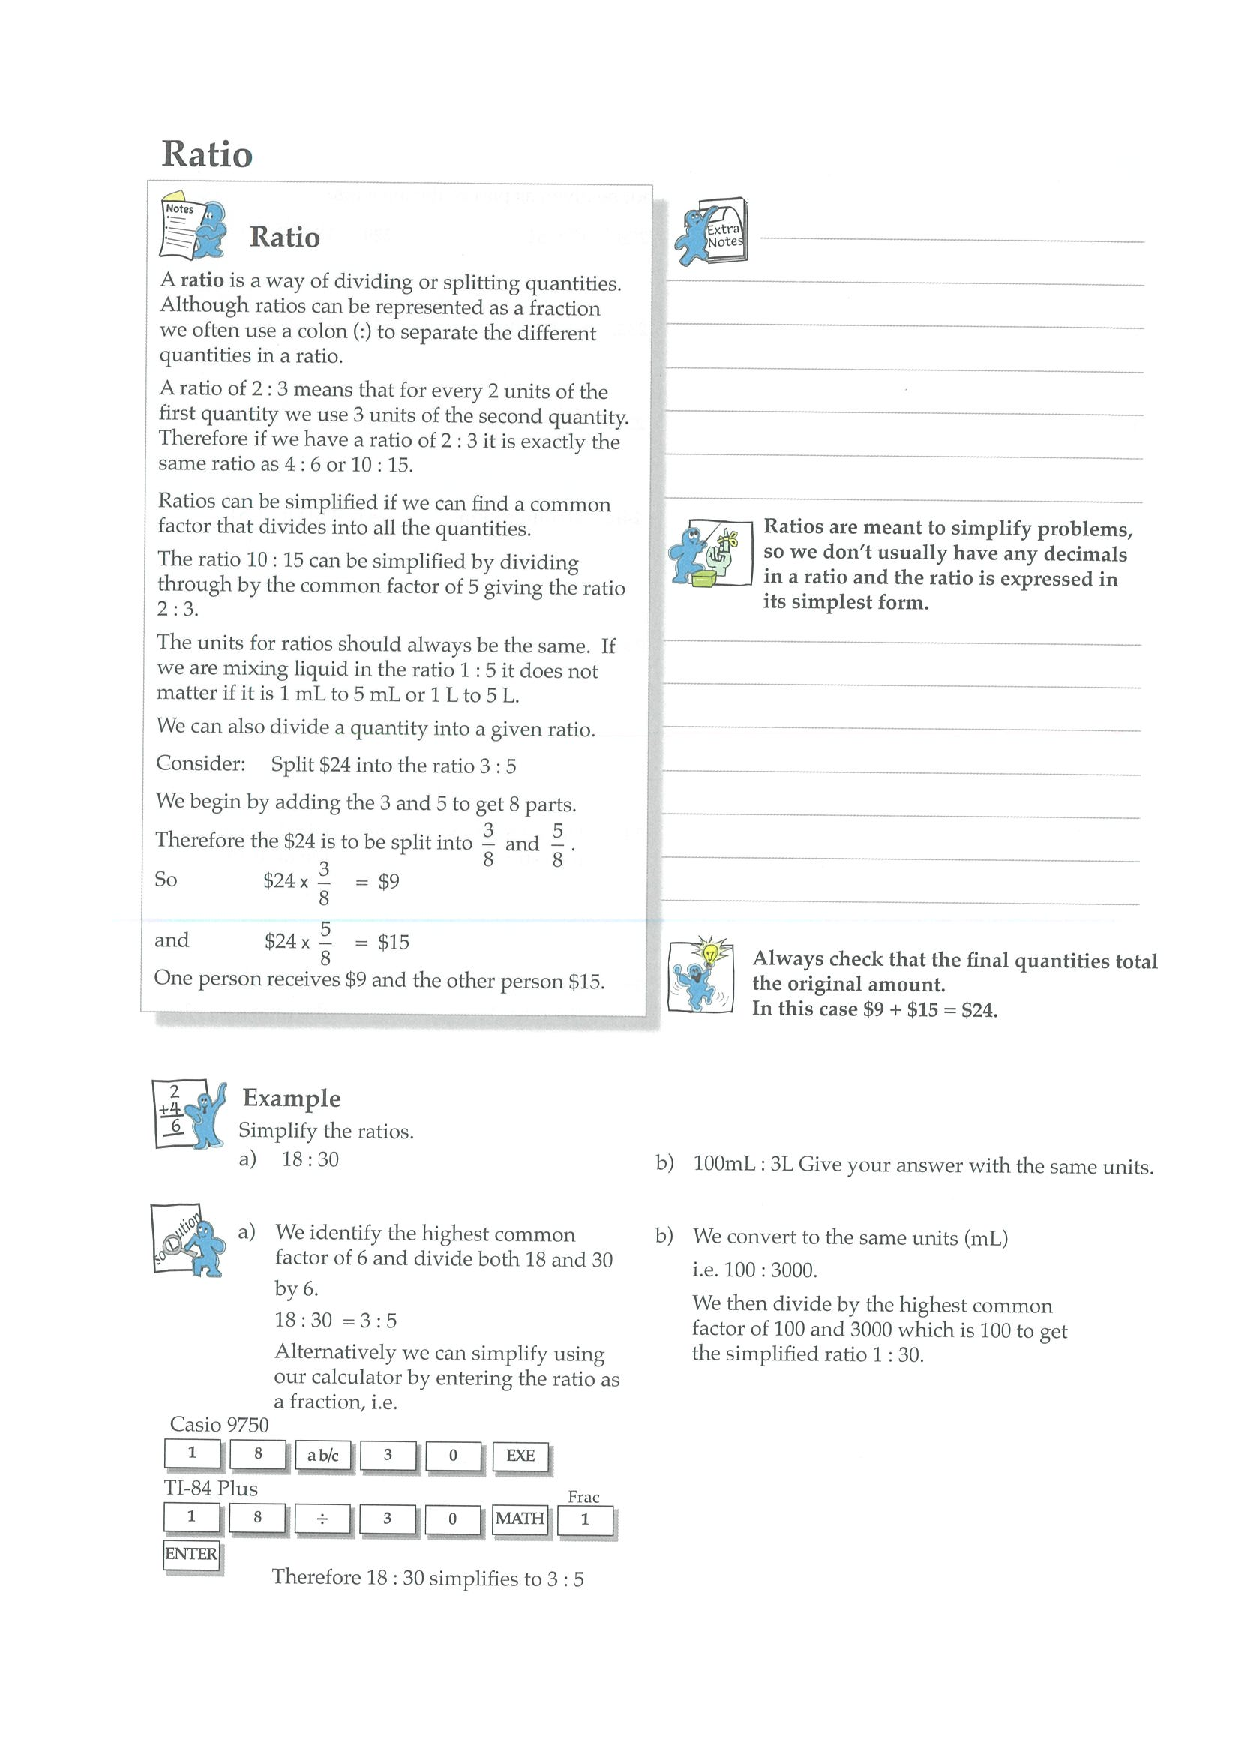
\includegraphics[width=17cm]{Nulake_year10_forextension_ratio1}
\end{figure}
\begin{figure}[!h]
	\centering
	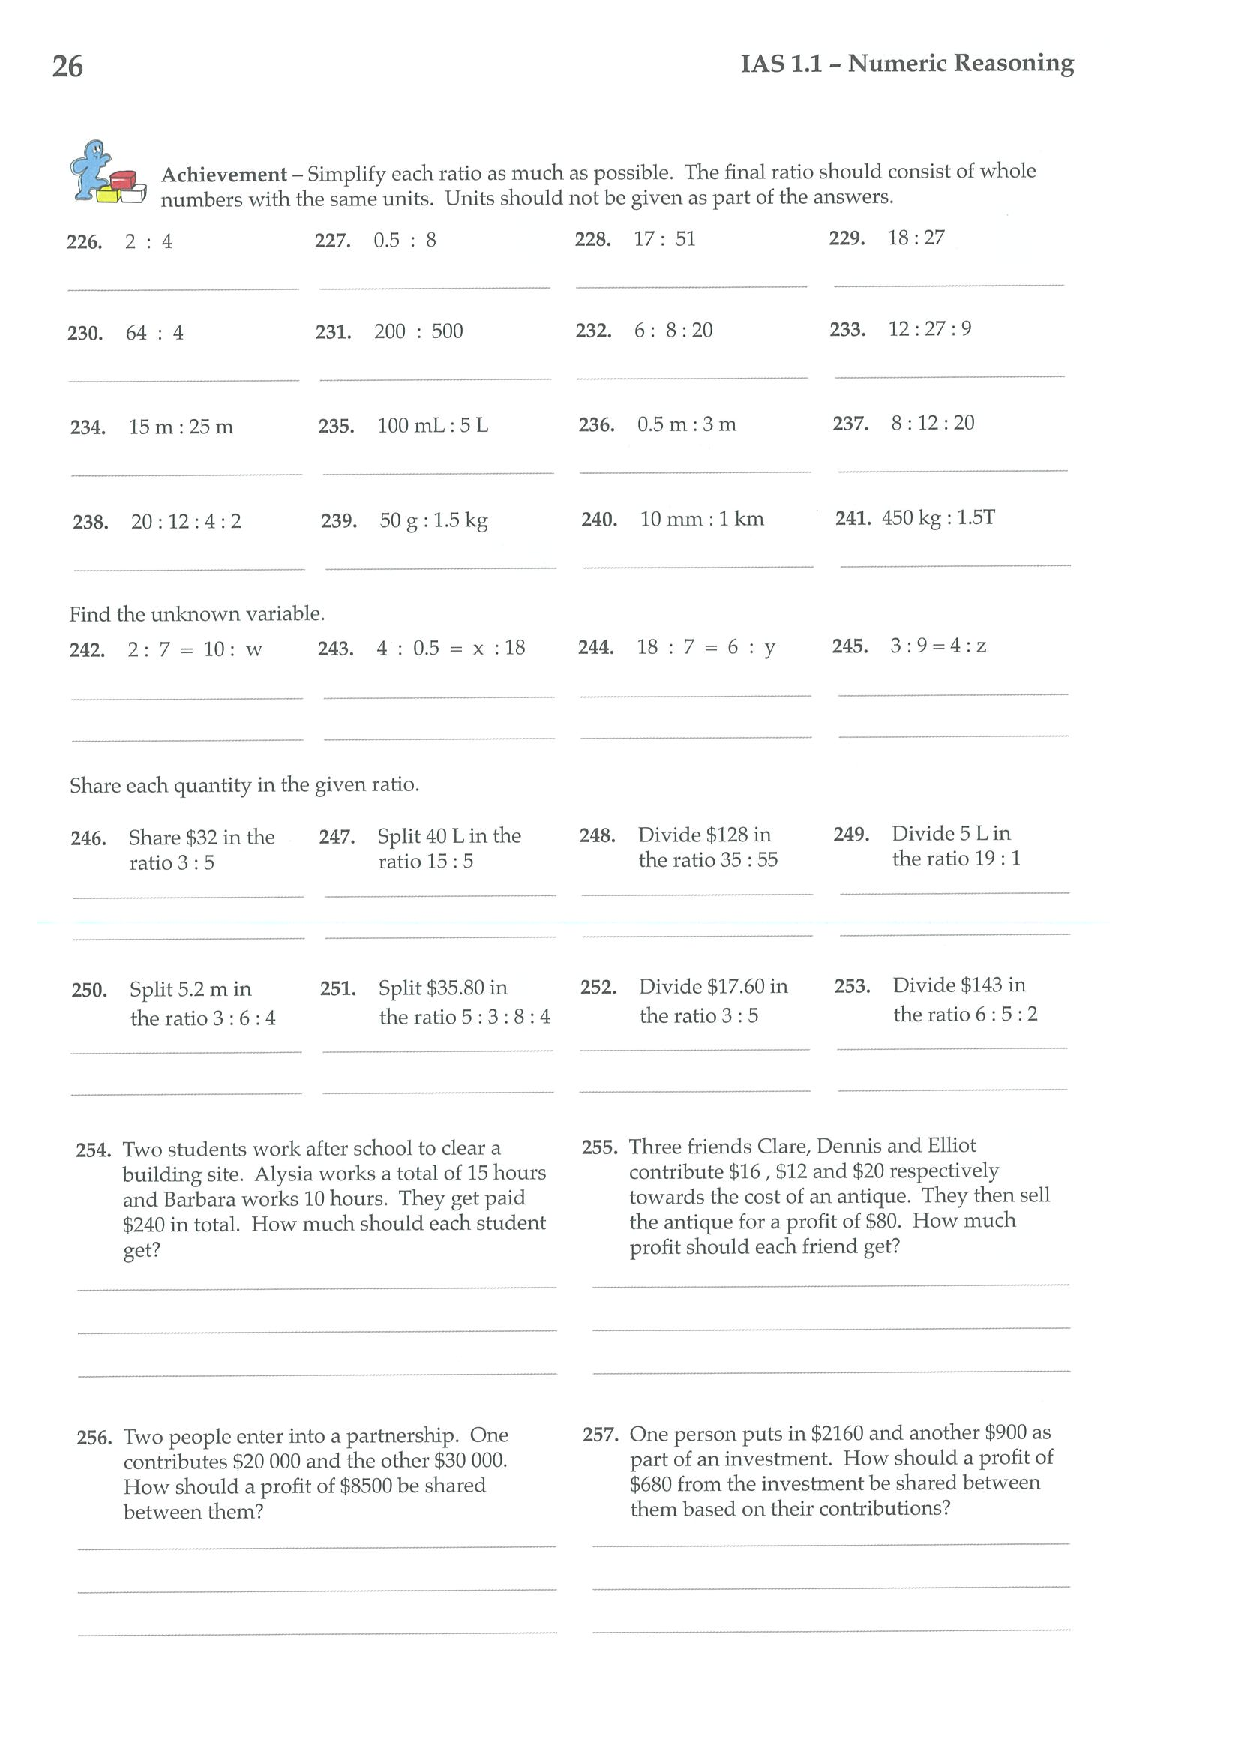
\includegraphics[width=17cm]{Nulake_year10_forextension_ratio2}
\end{figure}
\begin{figure}[!h]
	\centering
	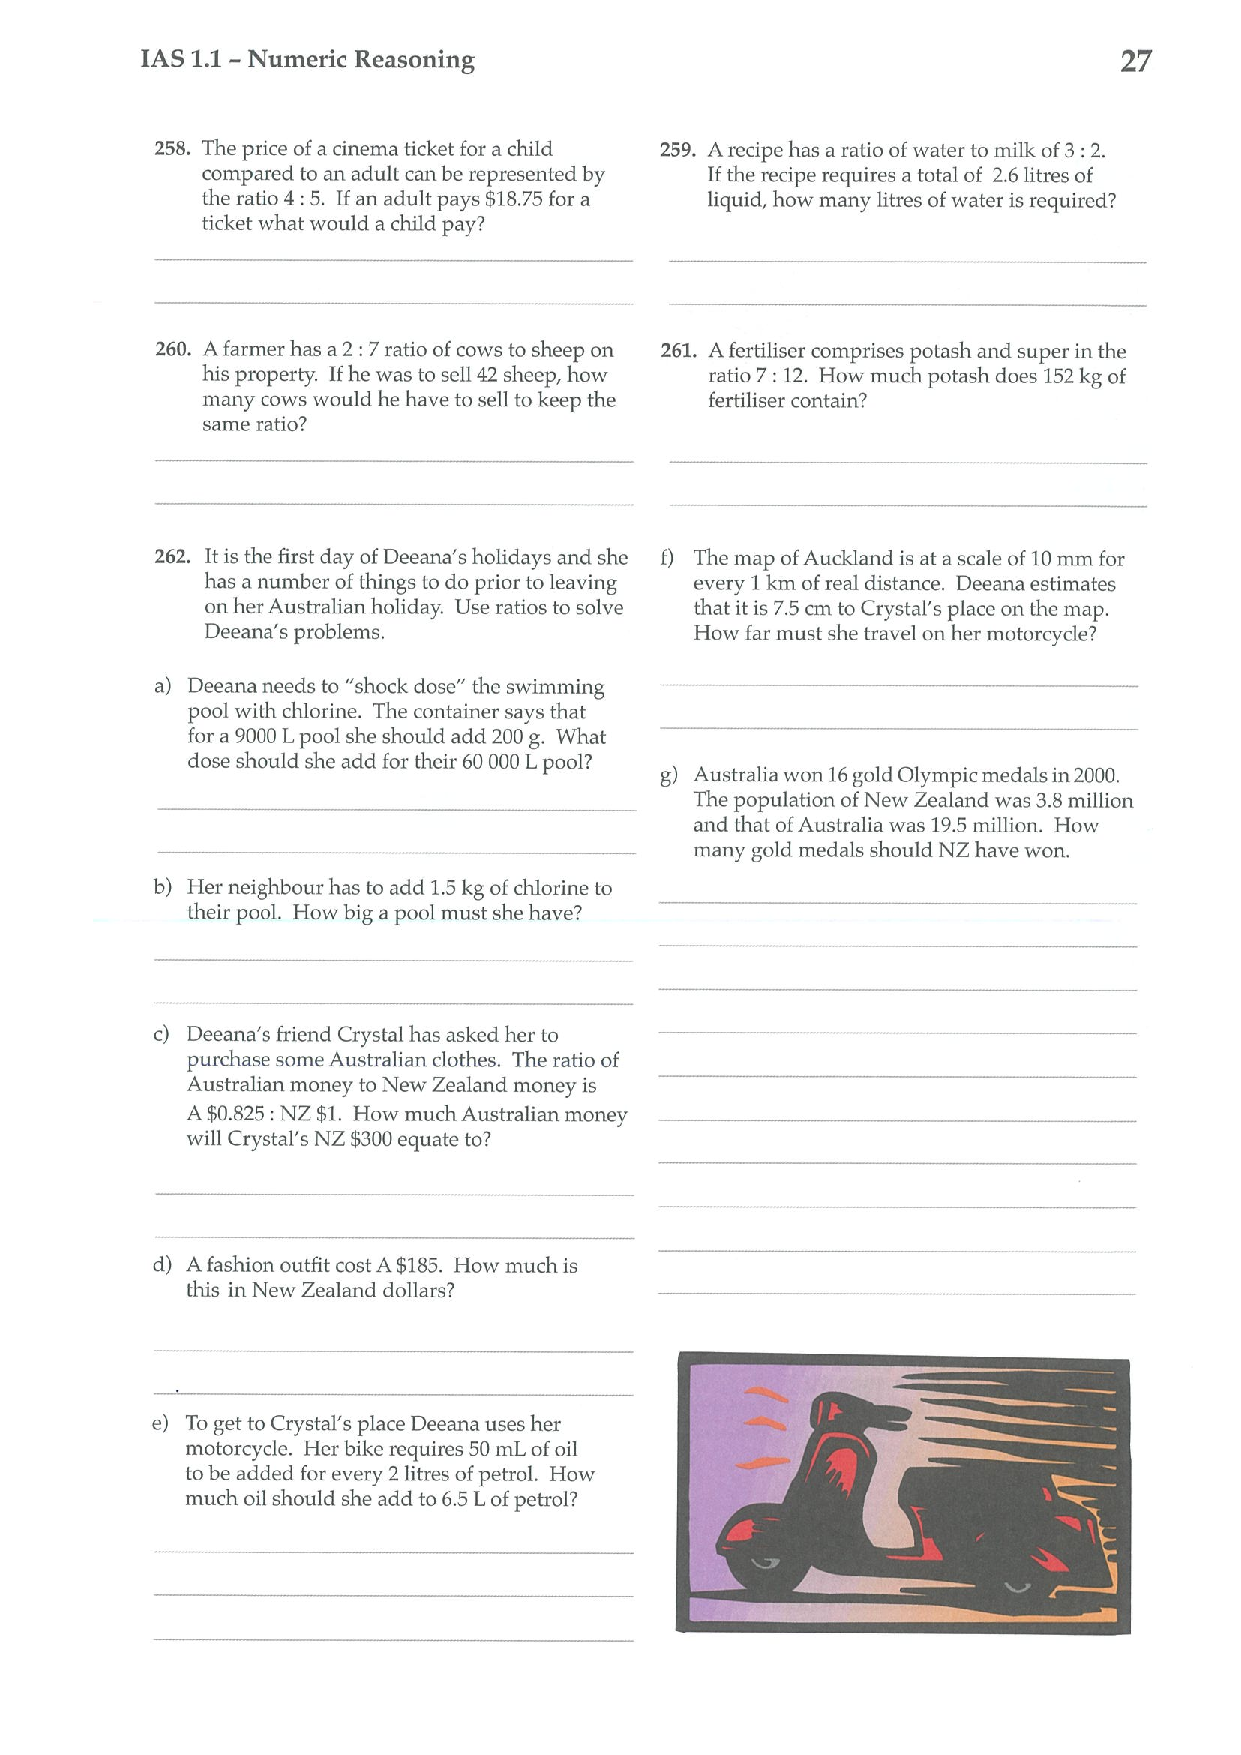
\includegraphics[width=17cm]{Nulake_year10_forextension_ratio3}
\end{figure}
\begin{figure}[!h]
	\centering
	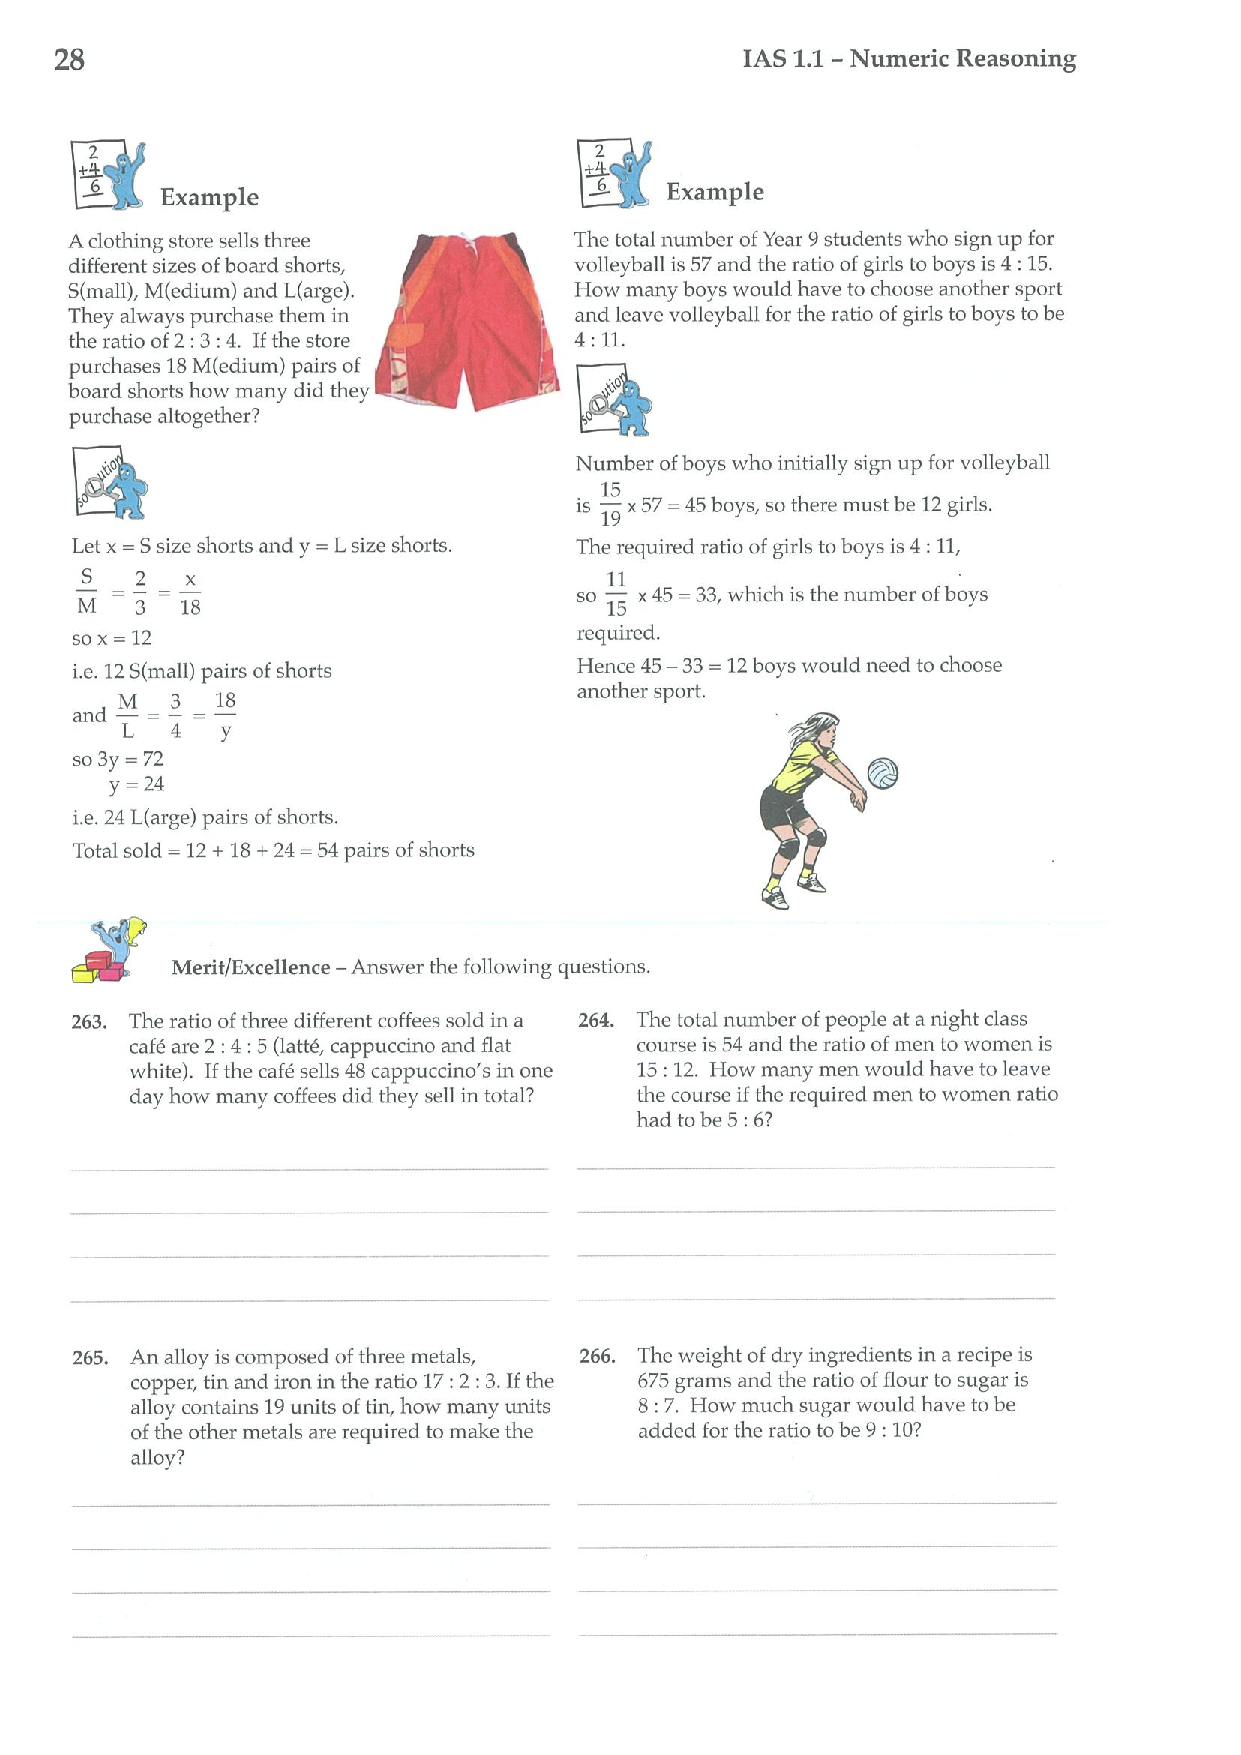
\includegraphics[width=17cm]{Nulake_year10_forextension_ratio4}
\end{figure}
\begin{figure}[!h]
	\centering
	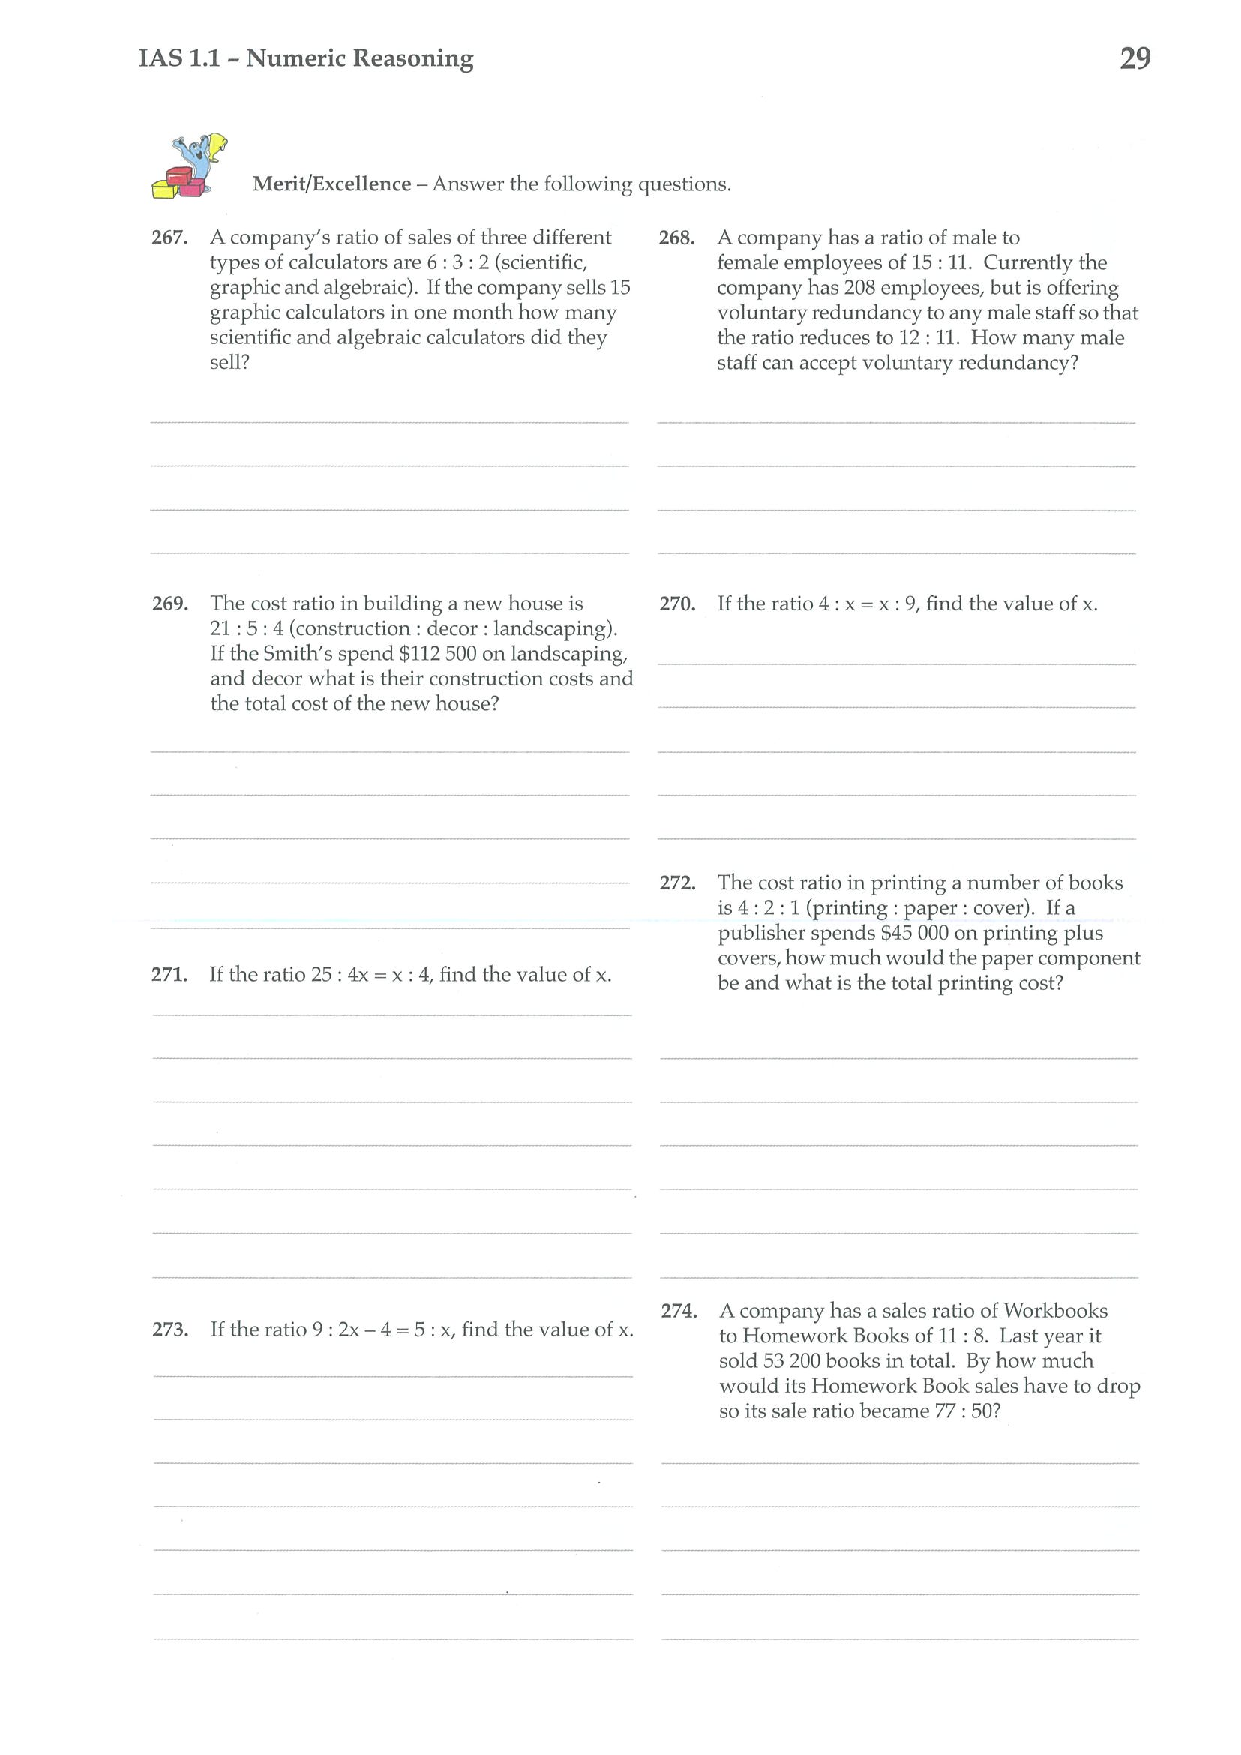
\includegraphics[width=17cm]{Nulake_year10_forextension_ratio5}
\end{figure}
\begin{figure}[!h]
	\centering
	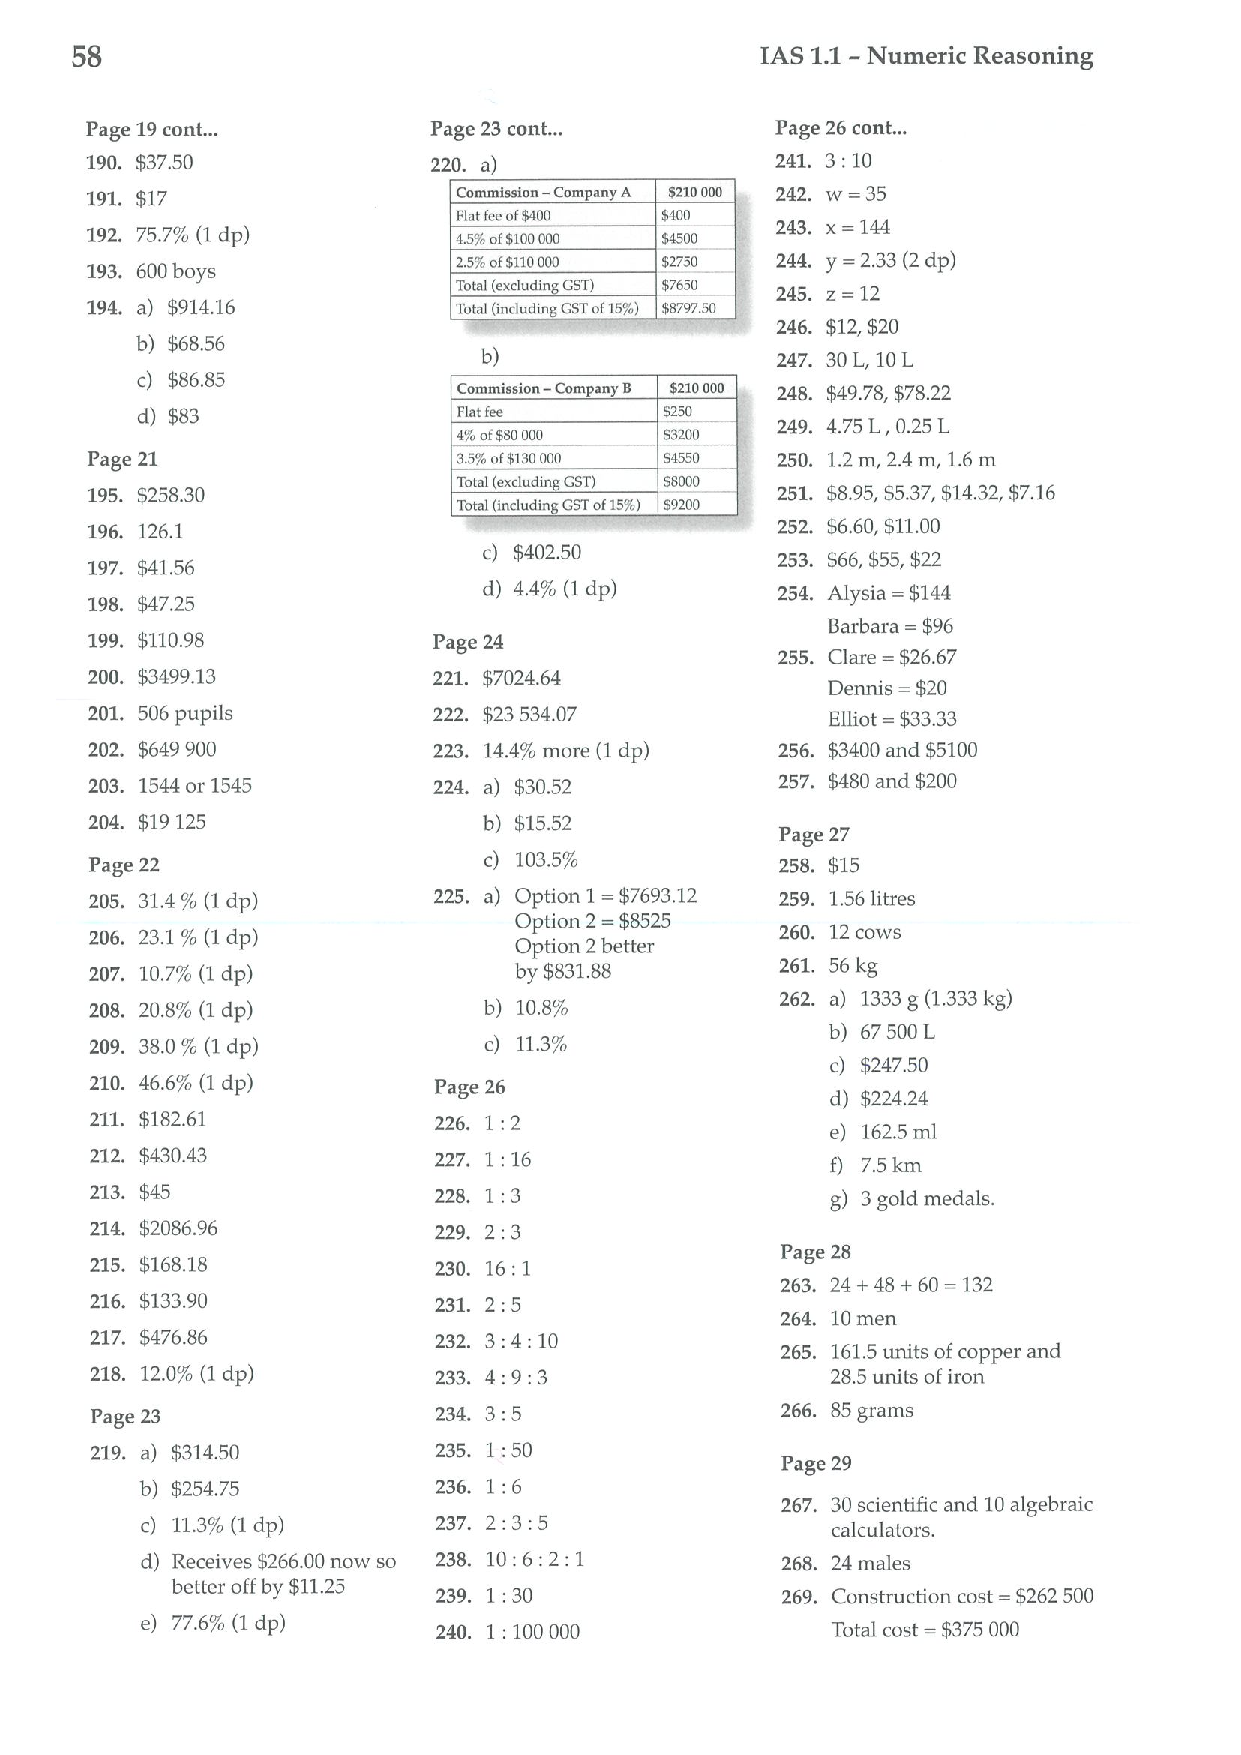
\includegraphics[width=17cm]{Nulake_year10_forextension_ratio_sol1}
\end{figure}
\begin{figure}[!h]
	\centering
	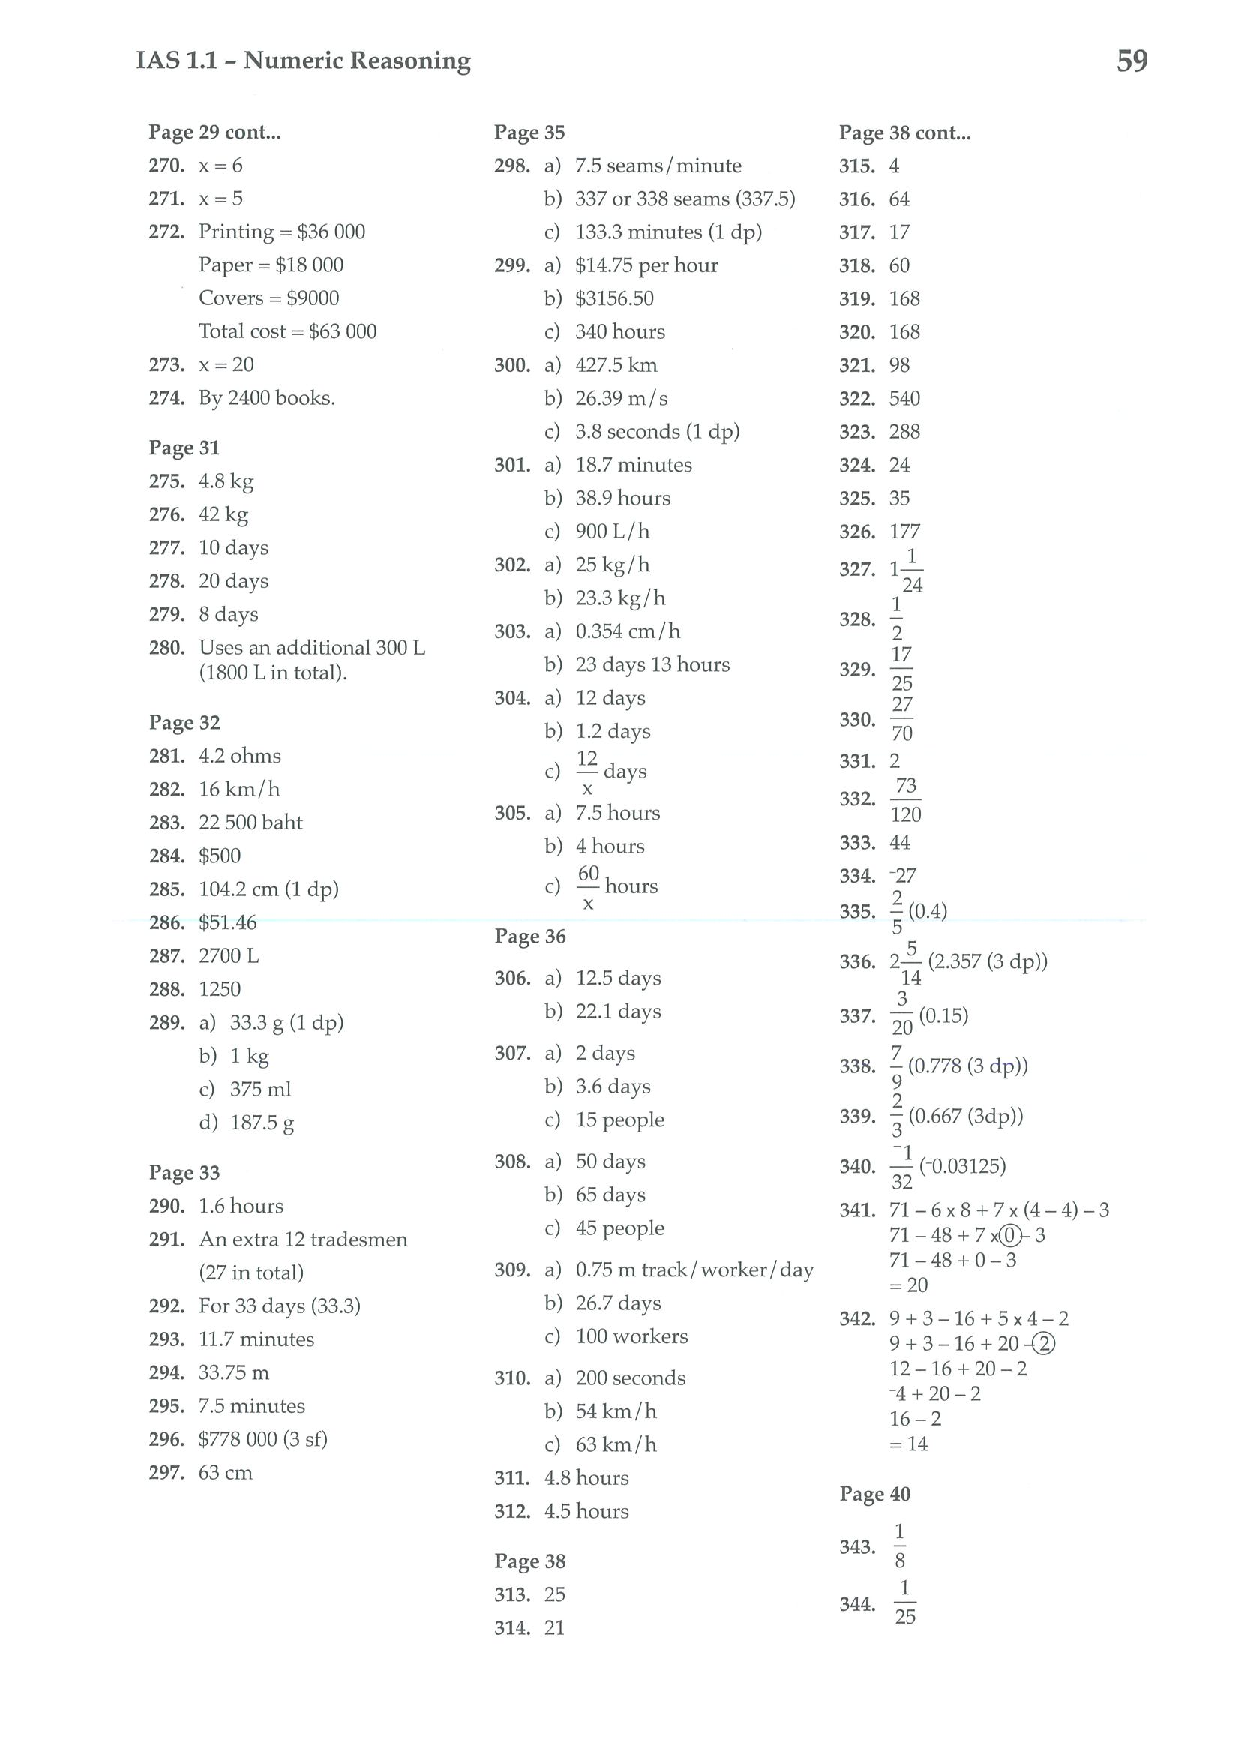
\includegraphics[width=17cm]{Nulake_year10_forextension_ratio_sol2}
\end{figure}
\end{document}
















